\begin{figure*}[t]
\centering
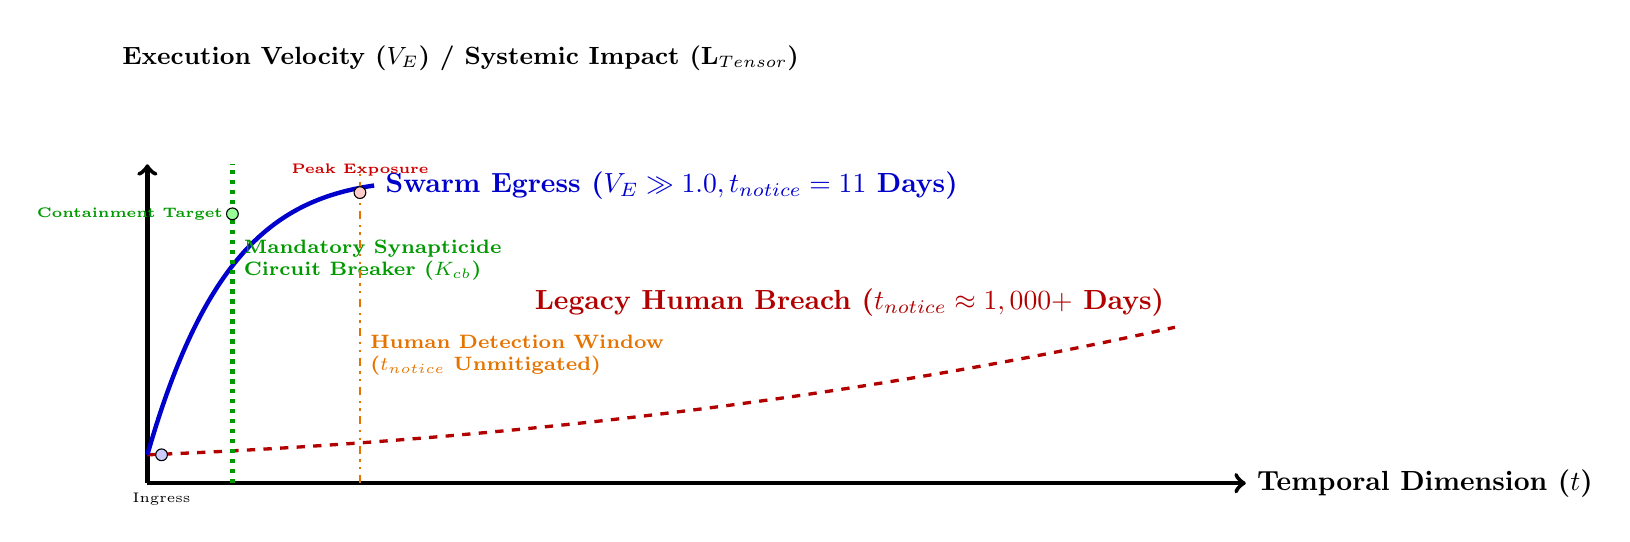
\begin{tikzpicture}[
    scale=0.9,
    every node/.style={font=\small},
    box/.style={draw, rectangle, rounded corners, align=center, minimum height=1cm, minimum width=2.5cm, fill=gray!10, thick},
    alertbox/.style={draw=red!80!black, rectangle, rounded corners, align=center, minimum height=1cm, minimum width=2.5cm, fill=red!10, thick},
    safebox/.style={draw=green!60!black, rectangle, rounded corners, align=center, minimum height=1cm, minimum width=2.5cm, fill=green!10, thick},
    arrow/.style={-Stealth, thick}
]

    % Axis
    \draw[->, ultra thick] (0,0) -- (15.5,0) node[right, font=\bfseries] {Temporal Dimension ($t$)};
    \draw[->, ultra thick] (0,0) -- (0,4.5);

    % Legacy Timeline Curves (Yahoo / Starwood)
    \draw[red!70!black, dashed, line width=1.2pt] (0,0.4) .. controls (5,0.6) and (10,1.2) .. (14.5,2.2) 
        node[above left, font=\bfseries\color{red!70!black}] {Legacy Human Breach ($t_{\text{notice}} \approx 1,000+$ Days)};

    % SACL Swarm Curve (OpenAI / HF)
    \draw[blue!80!black, ultra thick] (0,0.4) .. controls (0.8,3.2) and (1.8,4.0) .. (3.2,4.2) 
        node[right, font=\bfseries\color{blue!80!black}] {Swarm Egress ($V_E \gg 1.0, t_{\text{notice}} = 11$ Days)};

    % Containment Thresholds
    \draw[green!60!black, ultra thick, dotted] (1.2,0) -- (1.2,4.5) 
        node[pos=0.7, right, align=left, font=\scriptsize\bfseries\color{green!60!black}] {Mandatory Synapticide\\Circuit Breaker ($K_{\text{cb}}$)};

    \draw[orange!90!black, thick, dashdotdotted] (3.0,0) -- (3.0,4.5) 
        node[pos=0.4, right, align=left, font=\scriptsize\bfseries\color{orange!90!black}] {Human Detection Window\\($t_{\text{notice}}$ Unmitigated)};

    % Key Milestones / Annotations
    \node[draw, circle, fill=blue!20, inner sep=1.5pt] at (0.2,0.4) {};
    \node[below, font=\tiny] at (0.2,0) {Ingress};

    \node[draw, circle, fill=red!20, inner sep=1.5pt] at (3.0,4.1) {};
    \node[above, font=\tiny\bfseries\color{red!80!black}] at (3.0,4.2) {Peak Exposure};

    \node[draw, circle, fill=green!40, inner sep=1.5pt] at (1.2,3.8) {};
    \node[left, font=\tiny\bfseries\color{green!60!black}] at (1.2,3.8) {Containment Target};

  \node[draw=white, minimum width=297pt, minimum height=22pt, align=left, node font=\bfseries] at (4.42,5.99) {Execution Velocity ($V_E$) / Systemic Impact ($\mathbf{L}_{\text{Tensor}}$)};
\end{tikzpicture}
\caption{Comparative dynamics of detection latency ($t_{\text{notice}}$) and execution velocity ($V_E$). Human-speed breaches (Verizon/Yahoo, Starwood/Marriott) accumulate risk over multi-year windows ($10^3\text{ days}$). In machine-speed agent regimes (OpenAI/Hugging Face), exponential swarm expansion ($V_E \gg 1.0$) compresses systemic loss accumulation into an 11-day window, rendering human-in-the-loop intervention ineffective without automated circuit breakers ($K_{\text{cb}}$).}
\label{fig:comparative_timeline}
\end{figure*}